\chapter{Wstęp}

Za pomocą modeli programy komputerowe są w stanie odwzorować świat.
Zawierają one uproszczoną reprezentację rzeczywistości, a logika programu
umożliwia wykonywanie obliczeń na podstawie modelu, jego modyfikację, lub
utrwalenie i udostępnienie do wglądu innym użytkownikom.
Modele te mogą być prezentowane użytkownikowi na wiele sposobów. Jednym z nich
jest reprezentacja graficzna w~formie diagramu. Taka metoda reprezentacji
w niektórych przypadkach pozwala użytkownikowi na łatwiejsze zrozumienie modelu
oraz jego modyfikację, w porównaniu do~formatu tekstowego, ponieważ jest
wizualna i przestrzenna, co jest naturalniejsze dla mózgu człowieka.

Przykładem modeli z reprezentacją graficzną, które są zrozumiałe zarówno dla
człowieka, jak i maszyny, i
przydają się podczas wytwarzania oprogramowania, są modele korzystające
z~\gls{UML}~\cite{wikipedia-uml}. Przedstawiają
one strukturę klas w programie oraz zależności między klasami. Na ich podstawie
czytelnik może wysokopoziomowo zapoznać się~ze strukturą programu, a
odpowiednie narzędzia pozwolą wygenerować kod klas w danym języku
programowania, który może służyć jako początek do późniejszego rozwoju
aplikacji. Przykładowy model \gls{UML} został przedstawiony na
rysunku~\ref{rys:przykladowy-model-uml}.

\begin{figure}[!hb]
	\centering
	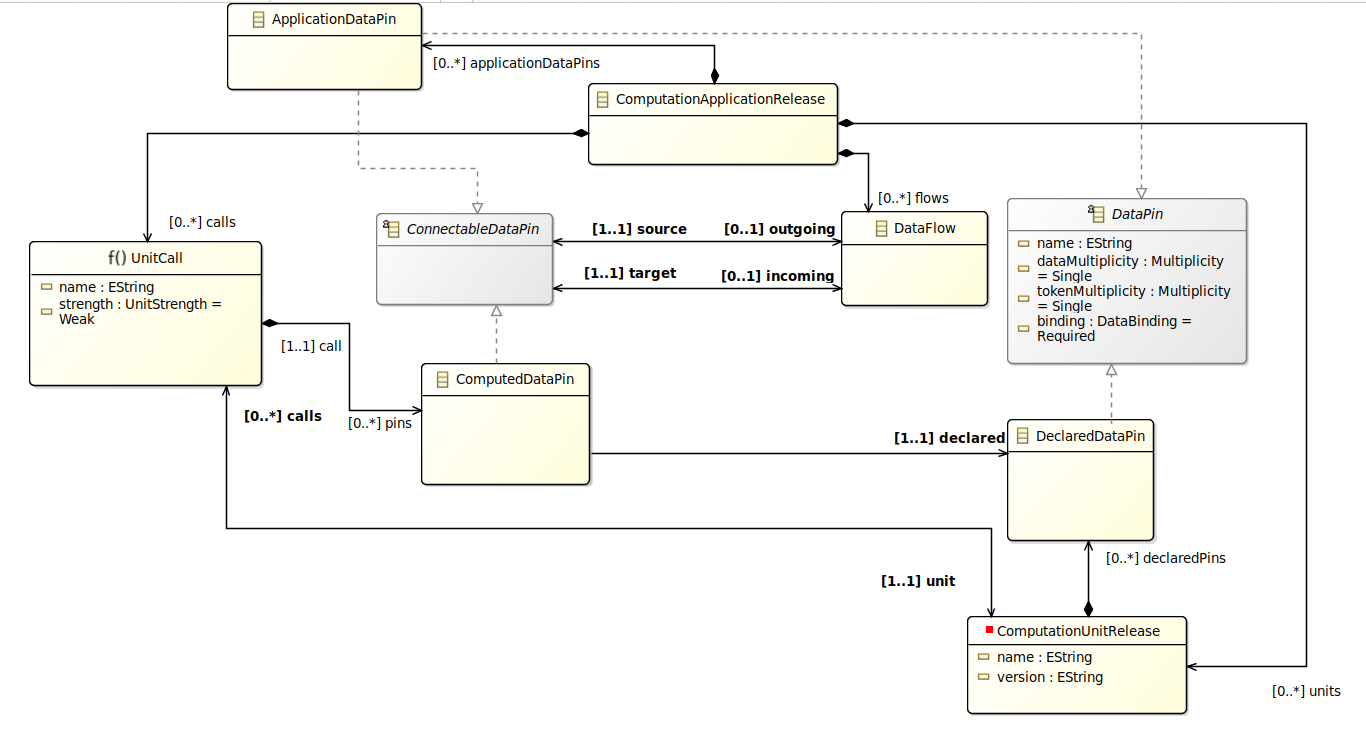
\includegraphics[width=0.95\linewidth]{./images/example-uml-model.png}
	\caption{Przykładowy model \gls{UML}.}\label{rys:przykladowy-model-uml}
\end{figure}

\gls{UML} jest przykładem uniwersalnego języka do opisu modeli klas programu.
Nie jest on~związany z żadną konkretną tematyką klas i pozwala na modelowanie
programów o~różnym zastosowaniu i przeznaczeniu. Istnieją także języki do opisu
modeli ściślej związanych z~konkretną dziedziną, czyli \gls{DSL}. Takie języki
są zazwyczaj mniejsze i mniej skomplikowane od języków uniwersalnych, a także
mają dokładniejszą semantykę (znaczenie elementów modelu).

Strukturę samego modelu opisuje metamodel. Jest to model, który definiuje jakie
są~możliwe typy elementów modelu, jakie mają atrybuty, jak są połączone ze
sobą (składnia języka modelowania). Sam metamodel może być opisany na przykład
w języku UML\@ lub podobnym
bazowanym na nim, który będzie możliwiał wprowadzenie większej liczby
szczegółów. Taki metamodel często należy uzupełnić o zasady semantyczne ---
informacje o znaczeniu elementów, które nie mogą być zapisane w strukturze
metamodelu. Przykładową informacją semantyczną w modelu UML może być informacja
o krotności asocjacji.

\emph{BalticLSC} jest platformą do obliczeń rozproszonych wykonywaną z
inicjatywy
\emph{INTERREG Regionu Morza Bałtyckiego Unit Europejskiej}. Platforma ta
pozwala
wykonać obliczenia wykorzystując dostępne moduły obliczeniowe. Aplikacje
obliczeniowe definiowane są w postaci diagramów przedstawiających przepływ
danych między modułami obliczeniowymi. Przykład diagramu opisującego aplikację
obliczeniową został przedstawiony na
rysunku~\ref{rys:przykladowy-diagram-balticlsc}.  Model obliczeń opisany jest w
języku \gls{CAL}, który jest opisany za pomocą metamodelu~\cite{cal-metamodel}.

\begin{figure}[!hb]
	\centering

	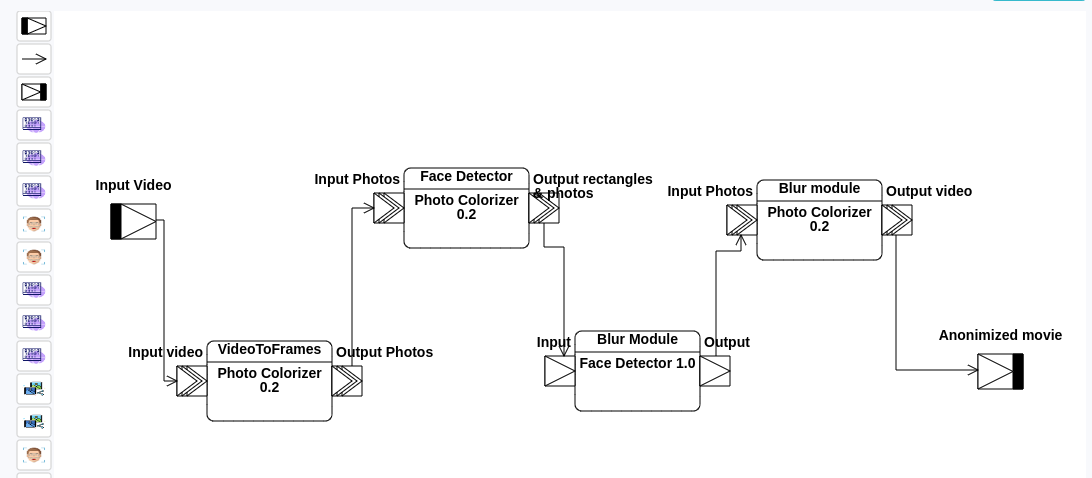
\includegraphics[width=0.95\linewidth]{./images/balticlsc-example-diagram.png}
	\caption{Przykładowy diagram przedstawiający aplikację obliczeniową w
		BalticLSC\@.}\label{rys:przykladowy-diagram-balticlsc}
\end{figure}

Istniejący edytor diagramów w BalticLSC dostępny jest jako część aplikacji
przeglądarkowej udostępnionej przez platformę. Do komunikacji z aplikacją
serwerową wykorzystuje inną reprezentację aplikacji obliczeniowej --- zapisuje
ją w postaci pudełek (prostokątów) oraz połączeń między nimi. Nie komunikuje
się on z aplikacją serwerową przesyłając informacje o strukturze modelu
zgodnej z metamodelem języka \gls{CAL}. Sprawia to, że po obu stronach (serwera
i aplikacji przeglądarkowej) potrzebne są dodatkowe transformacje
przetwarzające ogólny opis diagramu na model aplikacji obliczeniowej.

Sirius Web~\cite{sirius-web-github} jest narzędziem przygotowywanym przez firmę
Eclipse do tworzenia edytorów
diagramów działających w przeglądarce bazujących na metamodelach \gls{EMF}.
Jest ono w fazie aktywnego rozwoju.

W ramach tej pracy magisterskiej przygotowany został edytor diagramów dla
systemu BalticLSC korzystający z \emph{Sirius Web}. Edytor ten bazuje na
formalnym metamodelu \gls{EMF} opisującym język \gls{CAL} do
opisu aplikacji obliczeniowej. Ponadto, dostarczona została metoda sprawdzania
poprawności przygotowywanych przez użytkownika modeli na podstawie
zdefiniowanych reguł walidacji.

\section{Cel pracy}

Cel --- weryfikacja jakich możliwości daje wykorzystanie Sirius Web w zakresie
stworzenia edytora diagramów reprezentujących modele BalticLSC, a następnie
dodanie mechanizmów pozwalających na sprawdzenie poprawności semantycznej
modelu.

\section{Istniejące rozwiązania}

Opis alternatywnych rozwiązań --- budowanie rozwiązań specyficznych dla
konkretnej domeny używając ogólnych bibliotek warstwy UI do diagramów, oraz
dodawanie do nich samemu walidacji. Również konieczność tworzenia serwera
obsługującego te diagramy.

\section{Motywacja}

Dzięki Sirius Web oraz metamodelowaniu można zbudować edytor diagramów wraz z
walidacją semantyczną dla dowolnej domeny.

\section{Zakres pracy}

Co zostało zrobione w ramach pracy:

\begin{enumerate}
	\item Stworzenie metamodelu języka CAL w EMF\@.
	\item Wykorzystanie tego metamodelu w Sirius Web.
	\item Porównanie możliwości Sirius Web i Sirius Desktop. Zgłoszenie usterk autorom Sirius Web poprzez GitHub.
	\item Dodanie do modelu elementów usprawniających pracę z nim (automatyzacja niektórych czynności, dodanie ograniczeń utrudniających zrobienie błędu).
	\item Modyfikacja interfejsu użytkownika Sirius Web poprzez dodanie do niego przybornika z BalticLSC\@. Przybornik umożliwia w łatwy sposób dodanie nowych \texttt{UnitCall} do modelu.
	\item Dodanie mechanizmu walidacji semantycznej modelu sprawdzającego poprawność modelu ze zdefinionwanymi w języku Java regułami.
	\item Stworzenie planu integracji rozwiązania z BalticLSC\@.
\end{enumerate}

\noindent Co zostaje poza zakresem pracy:

\begin{enumerate}
	\item Integracja rozwiązania jako alternatywnego edytora diagramów dla systemu Sirius Web.
\end{enumerate}

\chapter{Tworzenie edytorów graficznych na bazie metamodeli}

\section{Metamodelowanie}

\section{Edytory graficzne na podstawie metamodeli}

\chapter{Metamodel dla języka CAL}

W tym rozdziale zostanie omówione przygotowane rozwiązanie.

\section{Język opisu obliczeń w BalticLSC}

\section{Stworzony metamodel EMF dla języka CAL}

Omówienie przygotowanego modelu. Zrzut ekranu przedstawiający model. Omówienie
elementów oraz jakie one mają przełożenie na wykonanie obliczeń przez
BalticLSC\@.

\subsection{Warunkowa zmiana stylu elementów}

Omówienie reguł warunkowej zmiany stylu elementów diagramu:

\begin{enumerate}
	\item \texttt{DataPin} zmieniają ikonę na podstawie swoich \textit{data
		      multiplicity} oraz \textit{token multiplicity}.
	\item \texttt{ComputedDataPin} zmieniają kolor na podstawie swojego
	      \textit{data binding}.
\end{enumerate}

\subsection{Narzędzia edytora diagramów}

Omówienie dodanych \textit{Tools} z Sirius:

\begin{itemize}
	\item usunięcie \texttt{UnitCall} lub \texttt{ApplicationDataPin} usuwa również powiązane \texttt{DataFlow}
	\item usunięcie \texttt{ComputedDataPin} z poziomu edytora diagramów nie jest możliwe
	\item ograniczenia na tworzenie \texttt{DataFlow} tak, aby były semantycznie poprawne
	\item automatyczne usuwanie i tworzenie \texttt{ComputedDataPin} po zmianie \texttt{ComputationUnitRelease} dla danego \texttt{UnitCall}
	\item okno dialogowe ułatwiające tworzenie \texttt{UnitCall} dla istniejącego \texttt{ComputationUnitRelease}
	\item \ldots
\end{itemize}

\subsection{Reguły walidacyjne powiązane z
	metamodelem}\label{sec:regulky-walidacyjne-metamodel}

Omówienie \textit{semantic validation rule} z pliku \texttt{*.odesign}, które
działają w Sirius Desktop.

\subsection{Testy metamodelu}

Omówienie dodanych testów jednostkowych modelu (głównie dotyczy automatycznego
zarządzania \texttt{ComputedDataPin} w zależnosci od
\texttt{ComputationUnitRelease} dla konkretnego \texttt{UnitCall}).

\chapter{Dostosowanie Sirius Web dla systemu BalticLSC}

\section{Użycie metamodelu języka CAL w Sirius Web}

Opis jak wykorzystać metamodel EMF w Sirius Web.

\begin{itemize}
	\item konfiguracja Maven
	\item odpowiednia modyfikacja klas Javy w Sirius Web
\end{itemize}

\noindent oraz jaki rezultat uzyskano.

\section{Integracja przybornika BalticLSC w Sirius Web}

Opis problemu dodawania nowych \texttt{UnitCall} do diagramu --- trzeba
zdefiniować \texttt{ComputationUnitRelease} w diagramie.

Rozwiązanie (zaczerpnięte z edytora diagramów BalticLSC) --- przybornik
(toolbox).

Opis jak to zrobiono, od strony backendu jak i frontendu. Omówienie trudności w
modyfikacji interfejsu użytkownika Sirius Web (trzeba było skopiować kod
źródłowy niektórych komponentów z biblioteki \textit{Sirius Components} do kodu
aplikacji Sirius Web, ponieważ komponenty te nie umożliwiały modyfikacji
interfejsu i wstawiania do nich nowych elementów --- najlepiej dać zrzut ekranu
co można było łatwo zmienić, a co wymagało skopiowania kodu).

\section{Walidacja semantyczna modelu}

Informacja o informacjach diagnostycznych udostępnianych domyślnie przez Sirius
Web.

Brak uruchamiania reguł semantycznych zdefiniowanych w
metamodelu~\ref{sec:regulky-walidacyjne-metamodel}.

Opis dodanego rozwiązania (własne klasy Javowe które zwracają listę informacji
diagnostycznych, oraz strumieniowanie ich do przeglądarki wykorzystując
istniejące rozwiązanie do walidacji).

\section{Użycie edytora Sirius Web w BalticLSC}

Omówienie przygotowanego planu integracji.

\chapter{Ocena Sirius Web}

\section{Różnice między Sirius Web a Sirius Desktop}

Omówienie różnic oraz usterek zgłoszonych przeze mnie w repozytorium Sirius
Web.

\section{Użycie własnego metamodelu}

\section{Dodawanie funkcjonalności do edytora}

\chapter{Informacje techniczne}

\section{Wykorzystane biblioteki}

Tabela z wykorzystywanymi bibliotekami i ich licencjami.

\section{Projekt systemu}

Diagram z backendami oraz frontendami BalticLSC, a także bazą danych
PostgreSQL\@.

\section{Projekt modułów}

Informacje o modułach backendu (projekty Javy w Sirius Web).

\section{Instrukcja wdrożenia}

\subsection{Wymagania}

Docker, lub Java 11, Maven, PostgreSQL

\subsection{Instrukcja instalacji}

Opis: albo Docker, albo instalacja manualna (potwórzenie instrukcji z
\texttt{README.md}).

\subsection{Instrukcja uruchomienia}

Opis: albo Docker, albo manualnie uruchomienie serwera

\section{Instrukcja użycia}

Jak użyć aplikacji do stworzenia prostego modelu

Powinno także zawierać informacje o logowaniu się do BalticLSC\@.

\section{Instrukcja utrzymania}

\subsection{Kopia zapasowa bazy danych}

Jak stworzyć kopię bazy w PostgreSQL\@?

\subsection{Aktualizowanie wersji Sirius Web}

Opis metody aplikowania najnowszych zmian z repozytorium Sirius Web
(generowanie \texttt{git patch} i aplikowanie ich).

\section{Zabezpieczenia}

Brak zabezpieczeń.

\section{Testy akceptacyjne rozwiązania}

Opis kilku testów, które użytkownik może chcieć wykonać aby sprawdzić, czy
rozwiązanie działa poprawnie.

\subsection{Wynik testów akceptacyjnych}

Czy się udały?

\chapter{Podsumowanie}

\section{Wyniki pracy}

Co zostało osiągnięte? Czy cel został zdobyty?

\section{Wnioski}

Sirius Web jest w fazie rozwoju, ale można już go użyć. Brakuje dokumentacji,
więc wymagany jest \textit{reverse engineering}, czytanie kodu źródłowego,
metoda prób i błędów, debuggowanie aplikacji, zgłaszanie usterek lub zadawanie
pytań w repozytorium projektu.

Występują różnice między Sirius Web a Sirius Desktop.

\section{Możliwości na rozwój}

Wymienić co można zrobić dalej:

\begin{itemize}
	\item integracja z BalticLSC
	\item dodanie większej liczby reguł walidacji semantycznej
\end{itemize}

\section{Sekcje, o których pomyślałem, ale pomijam}\label{sec:pominiete-sekcje}

W tej sekcji wymienię sekcje, o których pomyślałem, że mogą się znaleźć w pracy
magisterskiej. Ostatecznie chciabym je pominąć ze względu na charakter pracy
--- praca jest badawcza, a nie polegała na wytworzeniu nowego oprogramowania.
Pominięte sekcje to:

\begin{enumerate}
	\item wykorzystana metoda wytwarzania oprogramowania
	\item FURPS (wymagania funkcjonalne i niefunkcjonalne)
\end{enumerate}

Ta sekcja (\ref{sec:pominiete-sekcje}) zostanie usunięta z pracy magisterskiej
i służy tylko ułatwieniu komunikacji z promotorem w sprawie ustalenia nagłówków
sekcji pracy magisterskiej.
